\documentclass[10pt, letterpaper, twoside]{article}
\usepackage{hyperref}
\usepackage{graphicx}
\graphicspath{ {./} }

\begin{document}

\title{Assignment 2 - Ames House Price Dataset}
\author{Hengjian (Henry) Jia}
\maketitle

% i) Background; ii) Dataset; iii) Analysis; iv) Conclusions

\section{Dataset}

The dataset I've chosen is the Ames House Price dataset (\url{http://jse.amstat.org/v19n3/decock.pdf}). This dataset is widely used in regression analysis tutorials, so is suitable for this assignment. It is collected by Dean De Cock from the Truman State University. The dataset contains the value of individual residential property in Ames, Iowa  from 2006 to 2010. The dataset contains 2930 observations and a number of explanatory variables.

Predicting house prices is obviously useful for a number of reasons. Estate agents can use this to accurately gauge prices for negotiating sales. Economists can use it to help gauge economic metrics. But, I've only got 2 pages so I can't rabbit on.

\section{Analysis}

\subsection{Regression}
The vanilla linear regression technique introduced in the lectures are absolutely hopeless here. The large number of variables caused the model to overfit wildly. Vanilla linear regression yields a root mean squared error (RMSE) of around \$19000, but a test set error of well over several million. There are multiple ways to remedy this. One method is to reduce the number of explanatory variables used in the regression model. The explanatory variables can be chosen by individually evaluating their correlation with the sale price, and then selecting only the variables with the highest correlation to use in the regression model. This can be visualised through plotting the number of highest correlation explanatory variables used, against the resulting RMSE. As shown in figure 1, by selecting the 50 highest correlated variables, a RMSE of just over \$30000 can be reached on the test set.

Another alternative would be to use This however, requires a regularisation coefficient $\lambda$ to be chosen. This is done by plotting the root mean squared error (RMSE) behaves as $\lambda$ varies (see figure 2).

Another viable methodology would be to use ridge regression, though this would require choosing a suitable regularisation parameter $\lambda$. This can chosen visually by plotting the value of $\lambda$ against the resulting RMSE shown in figure 2. This shows that an RMSE of just over \$30000 can be reached when $2^2 \leq \lambda \leq 2^7$.

\begin{figure}[h]
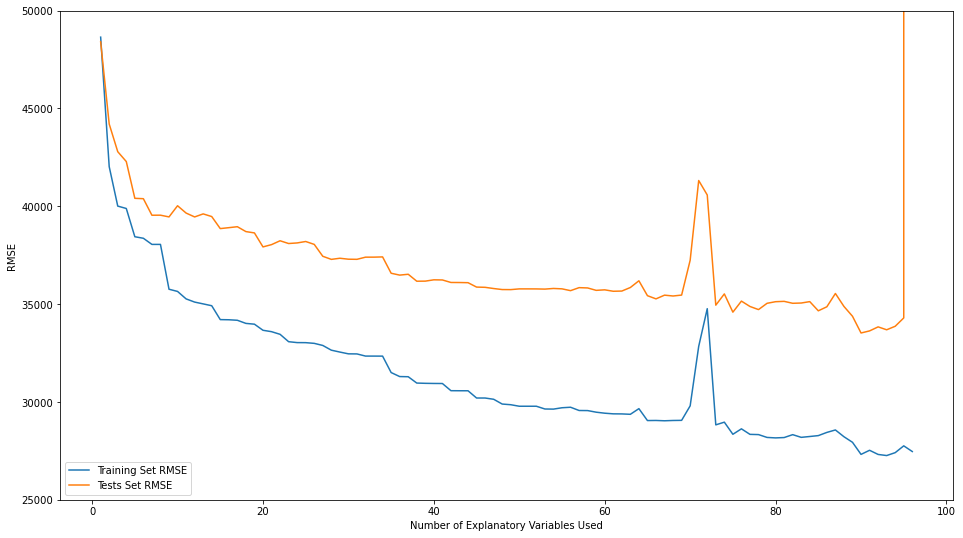
\includegraphics[width=10cm]{corr1}
\centering
\caption{Root mean squared error against number of explanatory variables}
\end{figure}

\begin{figure}[h]
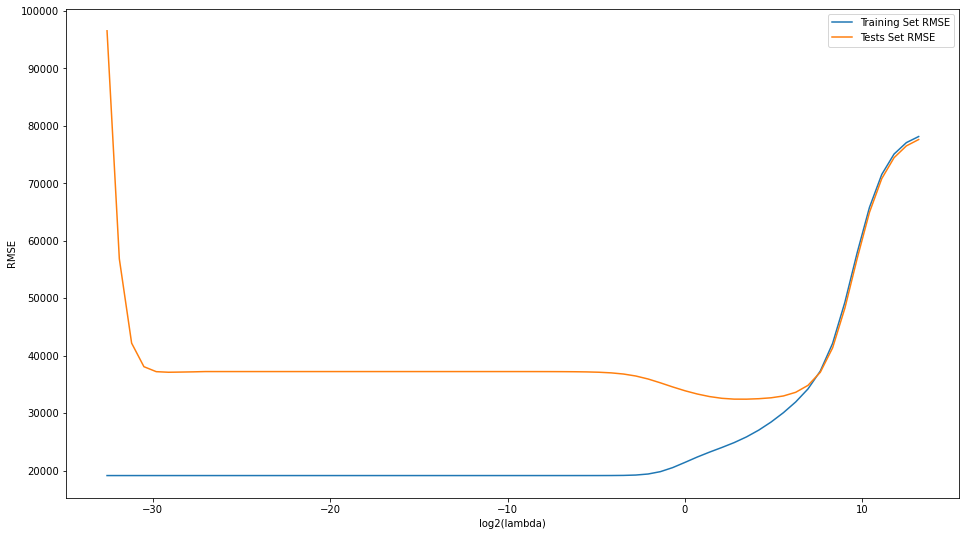
\includegraphics[width=10cm]{ridge}
\centering
\caption{Root mean squared error against $\log_2(\lambda)$}
\end{figure}

\section{Conclusion}

From this analysis, it can be concluded that house prices can be reasonably accurately gauged, through adapting the regression techniques in lectures. By choosing the explanatory variables intelligently or using advanced regression techniques, a suitable model can be inferred to predict house prices in Ames, Iowa with an RMSE of just over \$30000.

\appendix
\section{Appendix}
\subsection{Data Preprocessing}
The data needed a cleaning and preprocessing before any analysis. I first purged any explanatory variables which had more than 80\% missing data. This lead to 4 variables being purged: the type of road leading to the property, the quality of swimming pool the property had (if it had one), the quality of the property's fence (if it had one), and miscellaneous features of the property. This was followed by filling in any remaining missing entries with the mean for numerical variables, and the mode for categorical variables.

Finally, all numerical variables were shifted and scaled to have mean 0 and variance 1. All categorical variables were converted to a one hot representation.

\subsection{Ridge Regression}
Ridge regression seeks to minimise the modified version of the mean squared error
\[E(W) = \frac{1}{N} \sum_{k=1}^N (b + W^T x_k - y_k)^2 + \lambda ||W||_2^2\]
Where $\lambda$ is a hyperparameter. $\lambda$ controls how much we penalise the model for making $W$ large. This incentivises the model to not fully utilise all the input variables and reduces overfitting. The Bayesian interpretation of this is this is equivalent to applying a 0 mean Gaussian prior on $W$. By adjusting $\lambda$ we can balance overfitting and underfitting. If $\lambda$ is set to 0, this is equivalent to vanilla linear regression. If $\lambda$ is large, then the model tends to towards a horizontal straight line. 

\end{document}